\subsection{Trénování a dolaďování}
\label{subsec:training-fine-tuning}

Trénování LLM je procesem, během kterého model získává své schopnosti a znalosti z rozsáhlých dat.
Probíhá typicky ve třech fázích, z nichž každá plní odlišnou roli.
Celý proces trénování a následného nasazení modelu je schematicky znázorněn na \figref[obrázku]{fig:llm-training-pipeline}.
Výsledkem celého tří krokového procesu je model, jehož výstupy jsou věcnější, bezpečnější a lépe odpovídají záměru uživatele.

\subsubsection*{Předtrénování (pre-training).}
Předtrénování je výpočetně nejnáročnější fází celého procesu.
Model je trénován na stovkách miliard tokenů ze zdrojů jako jsou webové stránky, knihy, vědecké články nebo veřejné repositáře zdrojového kódu.
Trénovací data jsou nejprve tokenizována, tedy převedena na sekvence celočíselných identifikátorů odpovídajících jednotlivým slovním jednotkám nebo jejich částem (viz \secref[sekce]{subsubsec:tokenization}).

Cílem předtrénování je minimalizace záporné logaritmické věrohodnosti.
Model se snaží správně předpovídat každý token na základě předcházejícího kontextu:
\begin{equation}
    \mathcal{L} = -\sum_{t} \log P_\theta(x_t \mid x_1, \ldots, x_{t-1}). \label{eq:training-loss}
\end{equation}

Parametry modelu $\theta$ jsou iterativně aktualizovány algoritmem zpětného šíření chyby (\textit{backpropagation}).
V každém trénovacím kroku model zpracuje dávku sekvencí, vypočítá ztrátovou funkci a na jejím základě určí gradienty vůči všem parametrům.
Tyto gradienty jsou poté použity optimalizačním algoritmem, typicky variantou \textit{Adam}, k aktualizaci vah modelu směrem k nižší ztrátě.

Předtrénování vyžaduje enormní výpočetní prostředky.
Trénování modelů řádu desítek miliard parametrů probíhá na clusterech stovek až tisíců GPU po dobu týdnů až měsíců~\cite{brown-gpt3}.
Výsledkem je tzv.\ základní model (base model), který disponuje širokými jazykovými schopnostmi, avšak neumí přirozeně reagovat na pokyny uživatele.
Jeho tendencí je pouze pokračovat v textu na základě pravděpodobnostního rozdělení naučeného z trénovaných dat.

\subsubsection*{Instrukční dolaďování (supervised fine-tuning, SFT).}
Instrukční dolaďování přizpůsobuje základní model schopnosti řídit se pokyny.
Model je trénován na datové sadě tvořené páry instrukci a odpovědi, které byly typicky vytvořeny nebo zkontrolovány lidskými anotátory.
Příkladem takového páru může být instrukce \uv{Vysvětli rozdíl mezi zásobníkem a frontou} spárovaná s odpovídajícím strukturovaným vysvětlením.

Během SFT se model učí rozpoznávat formát konverzace, dodržovat zadané instrukce a generovat odpovědi ve stylu vhodném pro interakci s uživatelem.
Trénovací proces je technicky shodný s předtrénováním, stále se jedná o minimalizaci ztrátové funkce z rovnice~\eqref{eq:training-loss}.
Ztrátová funkce je však počítána pouze na tokenech odpovědi, nikoliv na tokenech instrukce.
Díky výrazně menšímu objemu dat, řádově tisíce až statisíce příkladů oproti miliardám tokenů při předtrénování, je tato fáze podstatně méně náročná na výpočetní prostředky.

\subsubsection*{RLHF}
Poslední fáze dále vylepšuje chování modelu na základě lidských preferencí.
Proces probíhá ve dvou krocích.

Nejprve je vytrénován pomocný model odměny (reward model).
Lidští hodnotitelé porovnávají dvojice odpovědí vygenerovaných modelem na stejný dotaz a označují, která z nich je lepší.
Z těchto preferencí se reward model naučí předpovídat numerické skóre kvality odpovědi.

Následně je hlavní model optimalizován pomocí algoritmu posilovaného učení, typicky PPO (Proximal Policy Optimization), tak, aby maximalizoval odměnu přidělenou reward modelem.
Současně je udržována blízkost k původnímu SFT modelu pomocí penalizace za příliš velké odchylky (KL divergence).
Tím se zabraňuje tzv.\ \textit{reward hackingu}, tedy situaci, kdy by model nalezl způsob, jak dosáhnout vysoké odměny bez skutečného zlepšení kvality odpovědí.

\begin{figure}[ht]
    \centering
    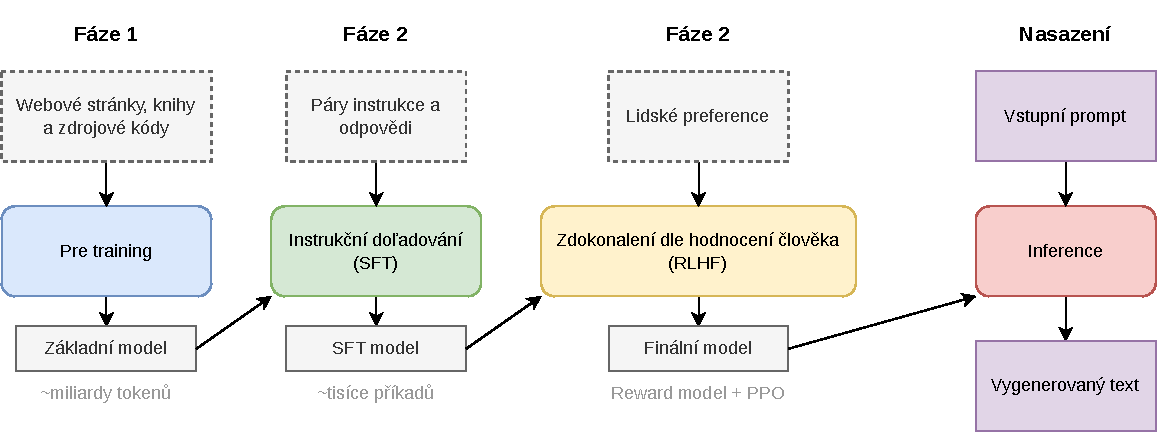
\includegraphics[width=1\textwidth]{resources/diagrams/model-training}
    \caption{Schéma celého procesu trénování LLM\@. Předtrénování, instrukční dolaďování a optimalizace před finálním nasazením pro inferenci.}
    \label{fig:llm-training-pipeline}
\end{figure}

\endinput